%!TEX root = thesis.tex

\chapter{Validity check for Markov analysis}

\subsection{Effect of dataset size} % (fold)
\label{sec:effect_of_dataset_size}
\begin{figure}[!t]
  \centering
   \subfloat[Hop and coverage for 44 players]{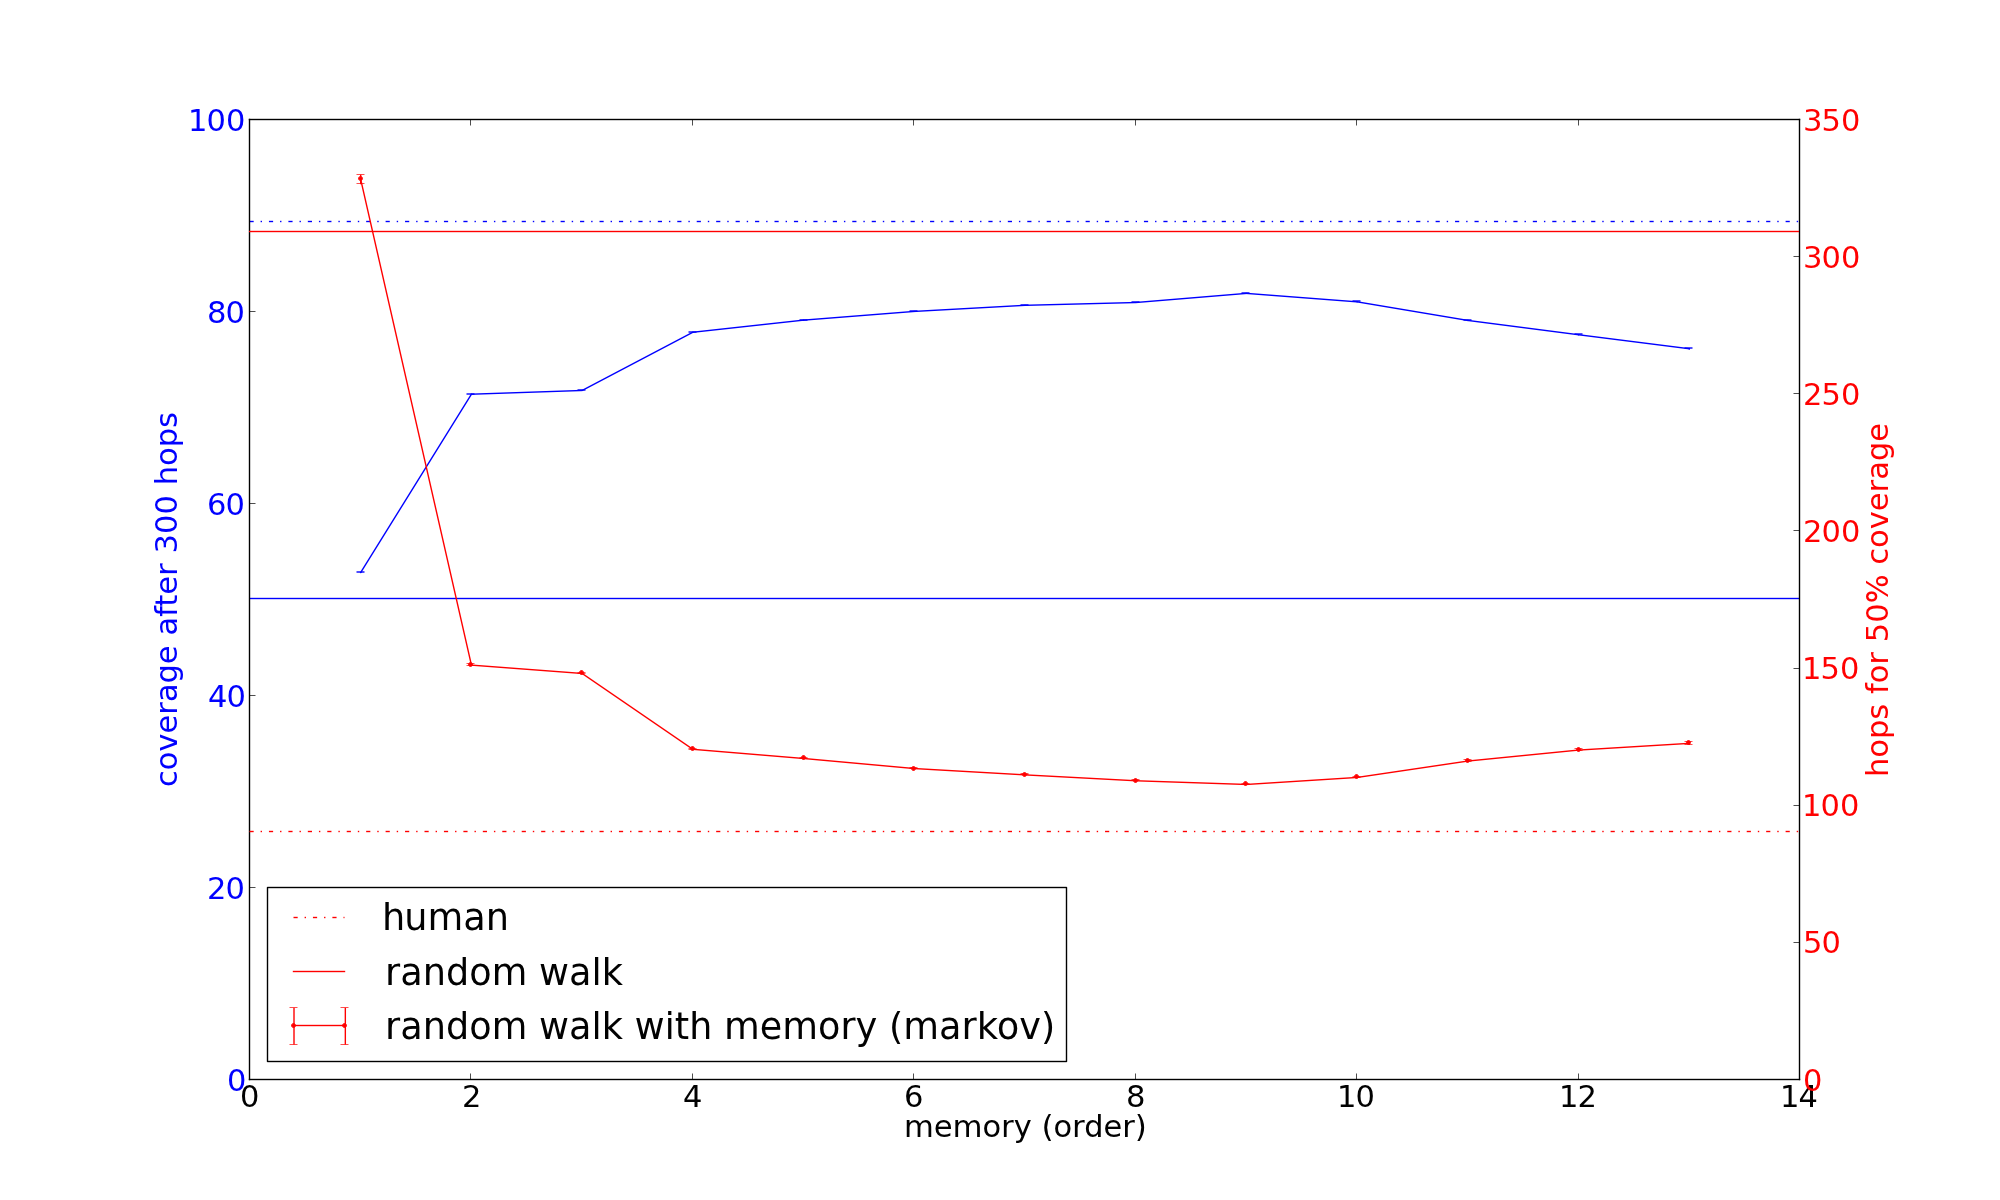
\includegraphics[width=\columnwidth]{44.PNG}}

  \subfloat[Hop and coverage for 22 players]{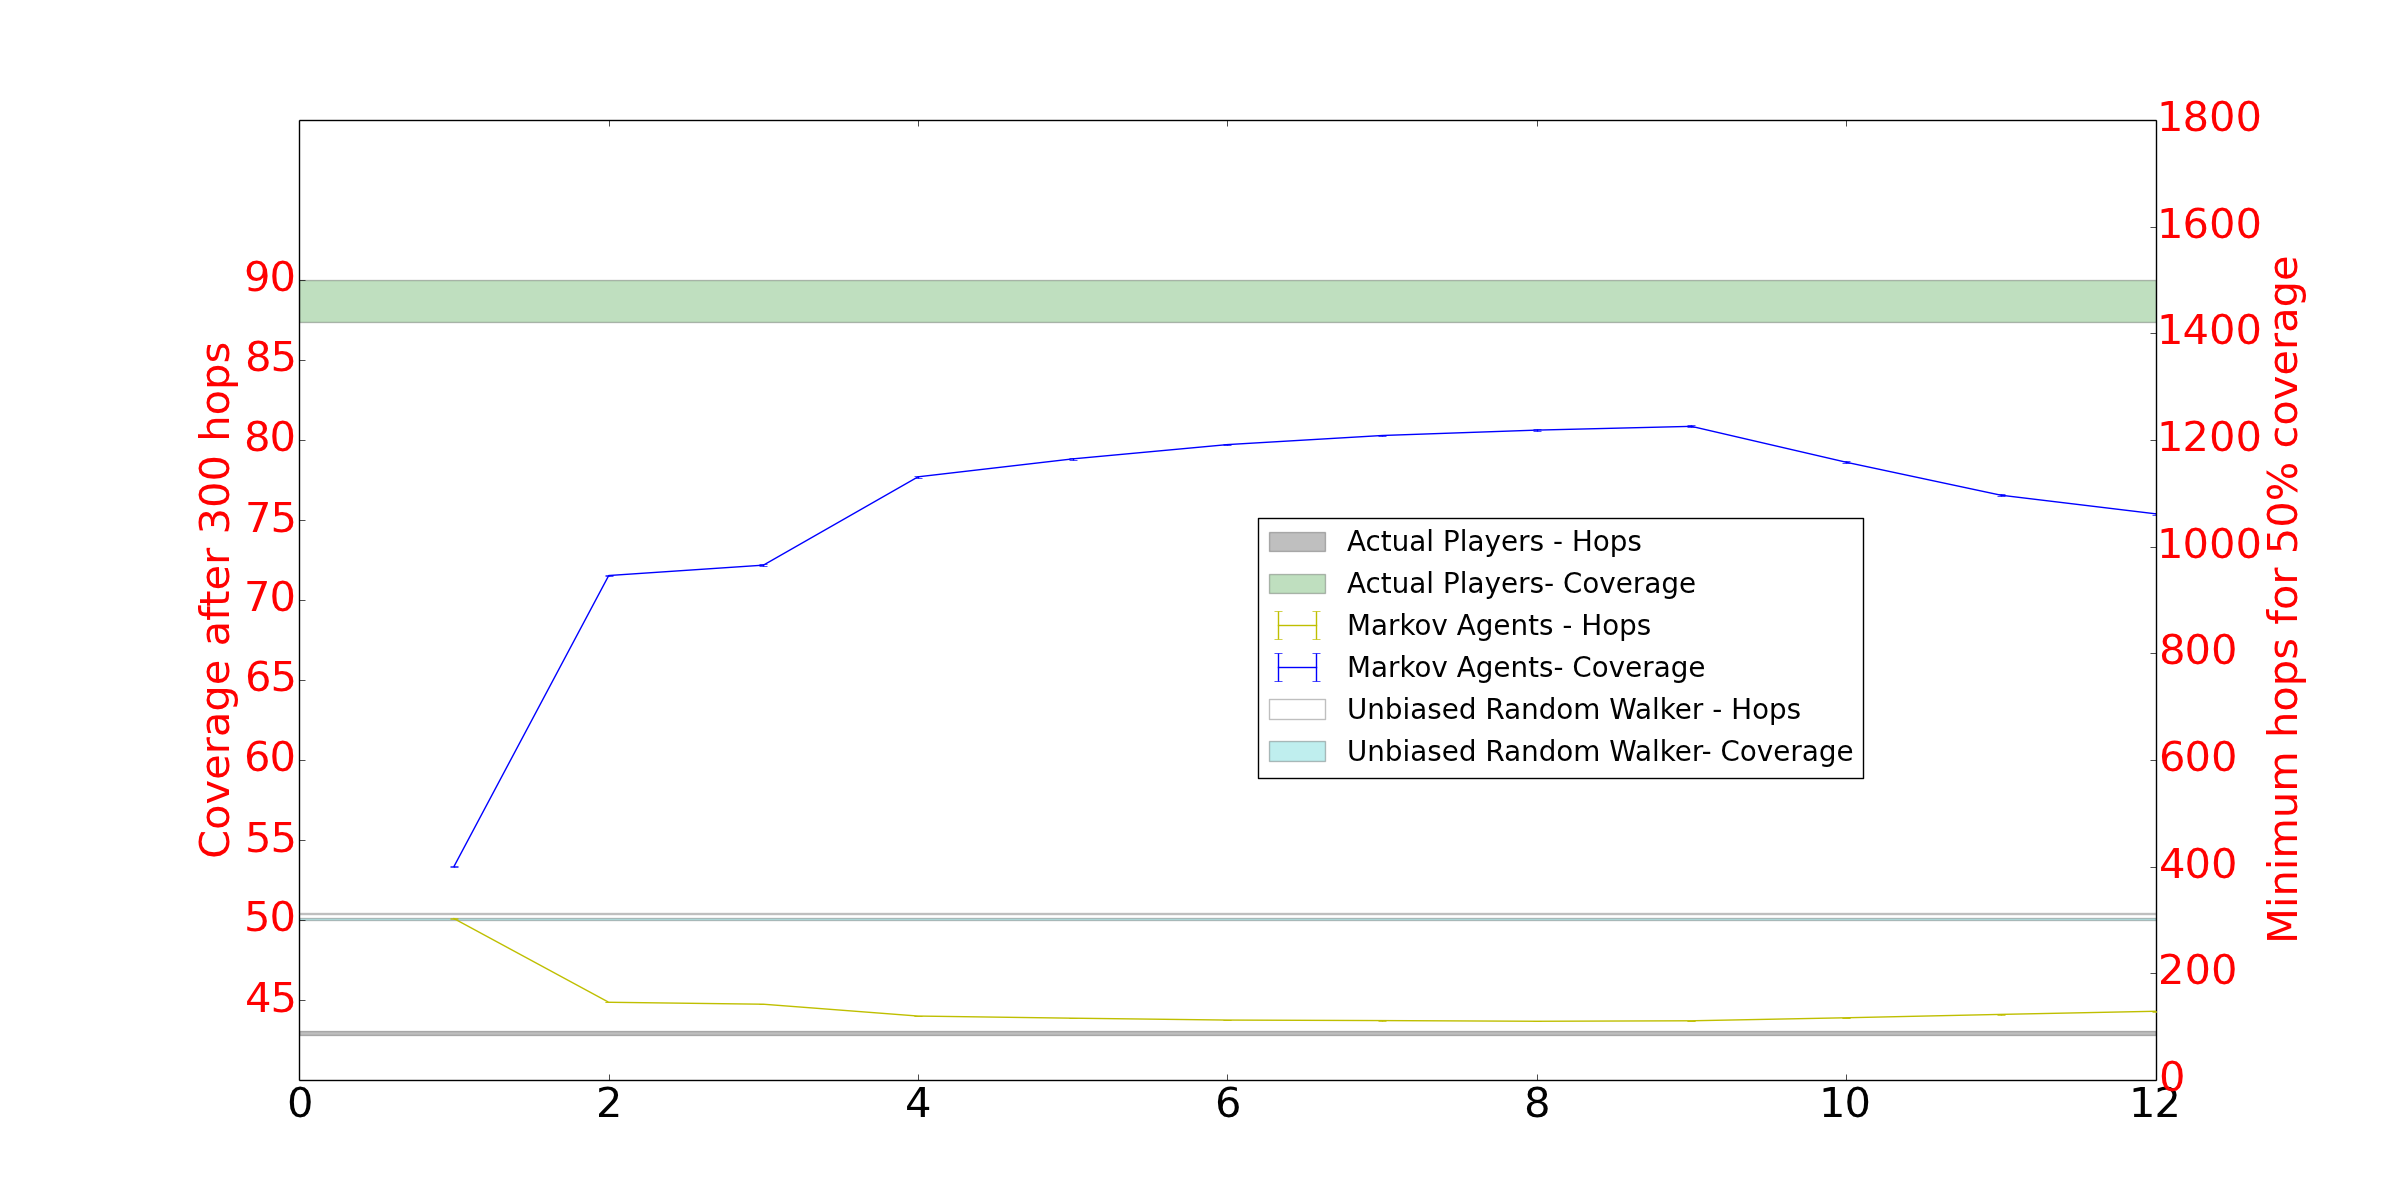
\includegraphics[width=\columnwidth]{22.PNG}}
  \caption{Hop and coverage graphs different size of datasets. Seems to indicate that the peak is not dependent on data size}
  \label{fig:hop_and_coverage_for_different_n}
\end{figure}




To check this, we hypothesized that if the peak does not change on doubling the dataset size then the pattern that is seen is not an artifact of the dataset size. We plotted the same graph for N=22 and N=44 and checked if there is a shift in the peak to a higher value. As shown in Figure~\ref{fig:hop_and_coverage_for_different_n} there is clearly no shift. The peak value still remains at 7-8 and starts dropping at 9.

\subsection{Decision base size at decision points} % (fold)
\label{sec:decision_base_size_at_decision_points}

\begin{figure}[tb]
    \begin{center}
        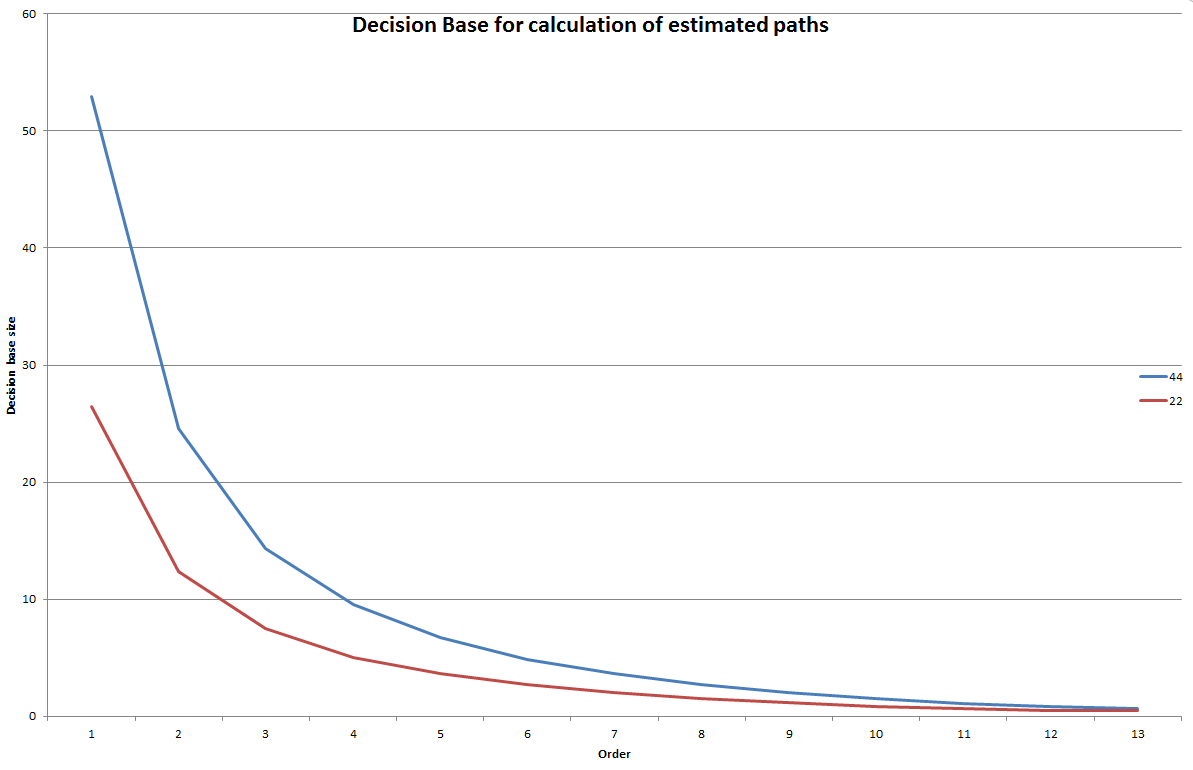
\includegraphics[width=\columnwidth]{decision-base-comparison.PNG}
    \end{center}
    \caption{Comparison of the decision bases}
    \label{fig:decision_base_comparison}
\end{figure}

Since the markov-data calculation is based on aggregating the actions of the agents at each decision point, the quality of the calculation is based on the amount of data available to make predictions. We refer to this as the \emph{decision base size} of the calculations.

For each node in each path generated the number of people that have actually made a decision at that point is calculated. We divide each of these values by the number of decisions that are possible at that point. So a single decimal value is obtained for each node of each path generated. The average of this over all nodes of a 300 hop path gives the \emph{path specific decision base}. 30,000 paths are generated the average of these path specific decision bases  gives an estimate of the decision base that is used, and in effect the reliability of the calculations in the preceding sections.

